\label{section:edge-area-chapter}
As the section before, we now want to show extensions where we split the surface of the triangle mesh likewise into regions around  edges and we draw all pixels in these regions with the same color (see Figure \ref{fig:min-area-edge}). This results in rhombus-shaped areas with constant color around each edge.

\begin{figure}[!h]
    \centering
    \minipage[b]{.5\linewidth}
    \centering
    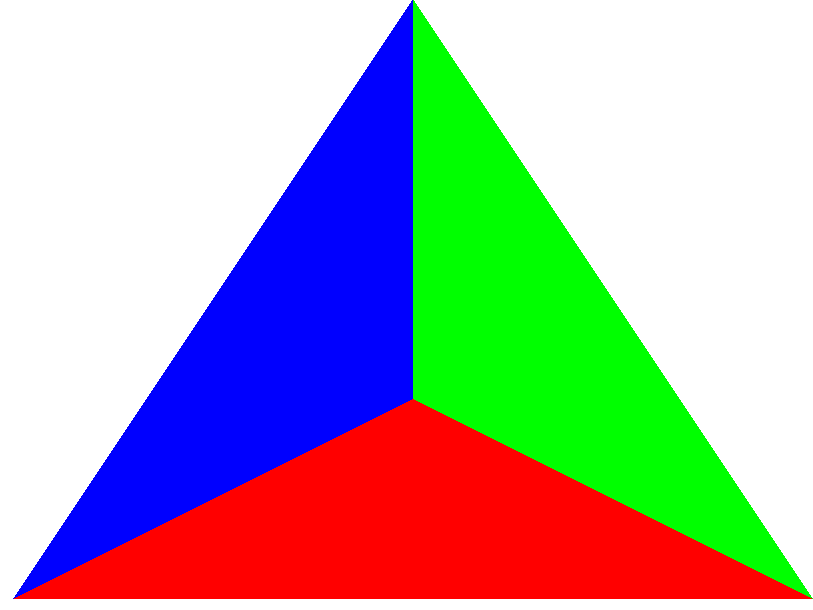
\includegraphics[scale=0.15]{images/min.png}
    \endminipage\hfill
    \minipage[b]{.5\linewidth}
    \centering
    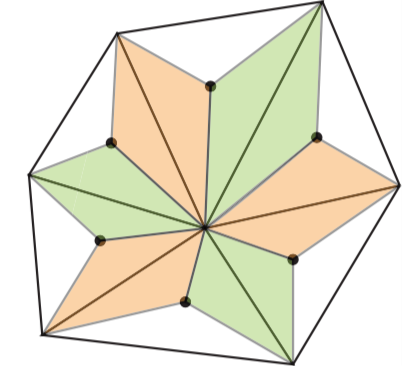
\includegraphics[scale=0.53]{images/edge-area.png}
    \endminipage
    \caption{On the left: Application of min diagram algorithm on a triangle. On the right: regions around edges.} \label{fig:min-area-edge}
\end{figure}

\subsection{Min diagram - Edge area} \label{section:min-diagram}
For each point in a triangle, we can easily determine its closest edge, which we use as a cue for coloring.
A different approach from interpolating, can be found coloring vertex areas based on the minimum barycentric coordinate.
The color is given by the region farthest from a vertex (Fig. \ref{fig:min-area-edge}, Pseudocode \ref{appendix:min-diagram}).

\subsection{Mean Curvature} \label{section:edge-struct} \label{section:mc-curvature}
Access to mesh edges requires to set up a list of edges over triangles. To avoid redundant data we have applied the convention that an edge would be counted only if it goes from a vertex with lower index into vertex with higher index in the list. A possible edge structure could look like the one in the pseudocode \ref{Pseudocode:edge}, where index\_v1 and index\_v2 are the vertex indices, norm\_edge is the length of edge, n1 and n2 are normals of adjacent triangles, cot\_alpha and cot\_beta are the cotangents of angles opposite to the edge, area\_t1 and area\_t2 are the areas of adjacent triangles.

\subsection{Constant Mean Curvature}
\textit{Constant mean Curvature} returns a constant color around each edge (see Fig. \ref{fig:armadillo-mean-edge}). Firstly it calculates the mean curvature for each edge $E$:
$$H(E) = || E|| (\theta_E /2)$$
where $\theta_E$ is the angle between the two normals of $T_1$ and $T_2$. The mean curvature for each vertex $V$ of a mesh is defined as:
$$H(E) = \frac{1}{2\mathcal{A}_{Barycentre}} \sum_{i = 1}^n ||E_i||(\theta_E/2)$$
where $\mathcal{A}_{Barycentre}$ is the area formed using barycenters. This value is then normalized. Every value is then mapped to positive or negative curvature, depending if the mesh at this edge is convex or concave, which can be known testing the determinant of the 3-by-3 matrix $M = [e, n_1, n_2]$ with those three vectors as
columns ($e$ is the edge $[W, V]$, $n_1$ is the normal of $T_1$ and $n_2$ is the normal of $T_2$). If $det(M) > 0$ then the mesh is convex at $[W, V]$ and the mean curvature would be positive, else the mesh is concave and the mean curvature would be negative. This technique of edge flat shading represents an alternative to the classic triangle flat shading.

\begin{figure}[!h]
    \centering
    \minipage[b]{.5\linewidth}
    \centering
    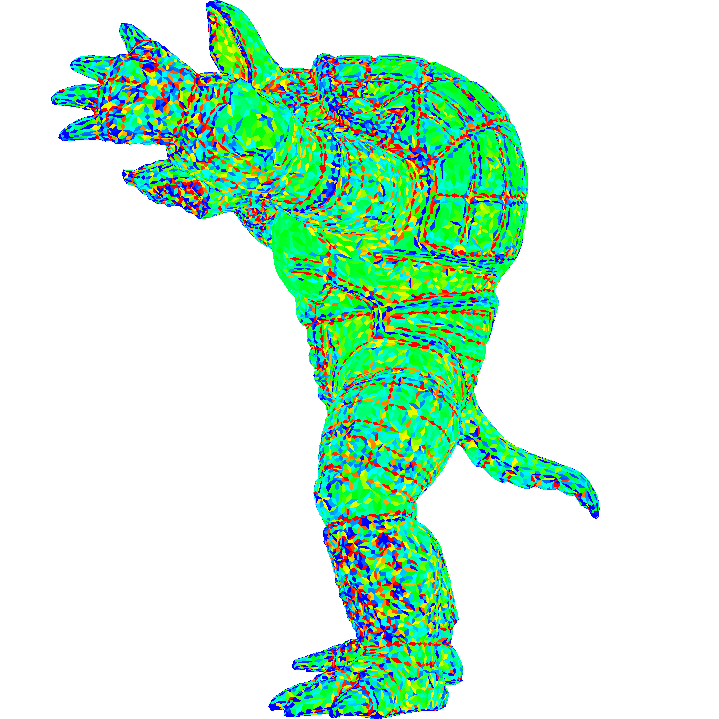
\includegraphics[scale=0.48]{images/mean-curvature-edge.png}
    \endminipage\hfill
    \minipage[b]{.5\linewidth}
    \centering
    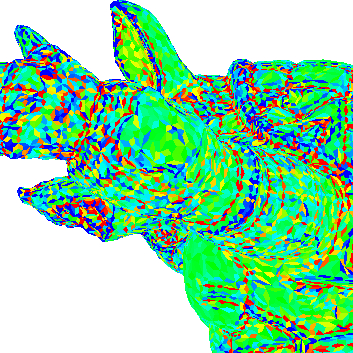
\includegraphics[scale=1.0]{images/mean-curvature-edge-detail.png}
    \endminipage
    \caption{Constant mean curvature} \label{fig:armadillo-mean-edge}
\end{figure}

\subsection{Gouraud Mean Curvature}
\textit{Gouraud mean Curvature} returns an interpolated color around each vertex. The main idea is to calculate the mean curvature $H(V)$ for each vertex $V$. In a mesh, every edge has two opposite angles (let us denominate these with $\alpha$ and $\beta$), the mean curvature per vertex is defined as:
$$H(V) = \frac{1}{2\mathcal{A}_{Mixed}} \sum_{i=1}^{n}(\cot \alpha_i + \cot \beta_i) (V - V_i)$$
where $V_i$ is one of the endpoints of the edge $E_i$.
These values are then interpolated using the automatic OpenGL interpolation resembling the classic Gouraud shading (see Fig. \ref{fig:armadillo-mean-vertex}).

\begin{figure}[!h]
    \centering
    \minipage[b]{.5\linewidth}
    \centering
    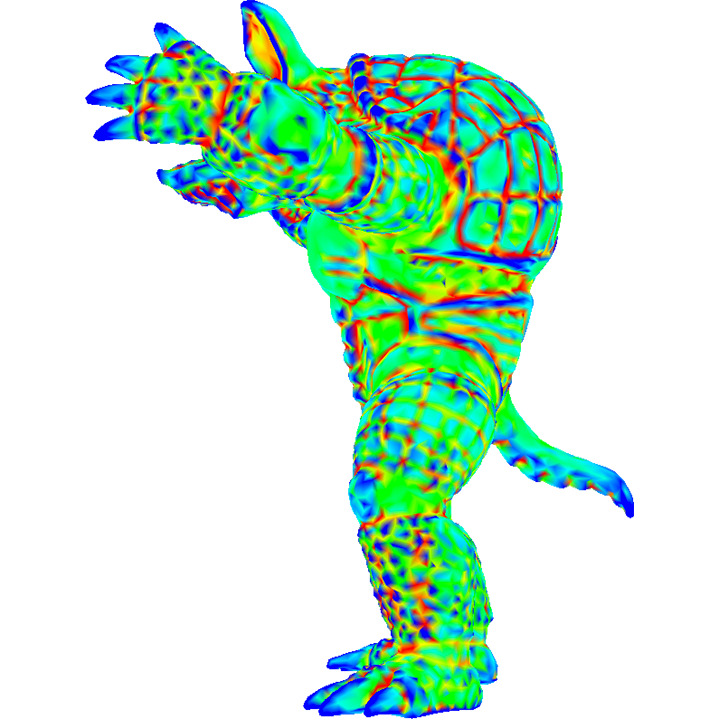
\includegraphics[scale=0.24]{images/mean-curvature-vertex.png}
    \endminipage\hfill
    \minipage[b]{.5\linewidth}
    \centering
    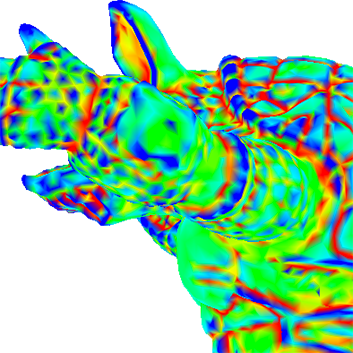
\includegraphics[scale=0.5]{images/mean-curvature-vertex-detail.png}
    \endminipage
    \caption{Gouraud mean curvature} \label{fig:armadillo-mean-vertex}
\end{figure}


\subsection{Evaluation and Comparison between constant mean curvature and gouraud mean curvature}
\textit{Constant mean curvature} is a curvature per
edge that returns a constant color around each edge
using the min diagram algorithm. The result is a noisy and sharped mesh with emphasized edges. This visualization could be helpful to show the quality of mesh triangulation and flows around surfaces. The flows are observable because edges are directed allowing the user to better analyze curvatures (see Fig. \ref{fig:armadillo-mean-edge}). \textit{Gouraud mean curvature}, on the other hand, returns more blurred meshes compared to the ones obtained with  \textit{Gouraud Gaussian curvature}. This smoothing is caused by the fact that mean curvature would be calculated per edge but in this case, we are averaging per vertex, this results in a loss of data (see Fig. \ref{fig:armadillo-mean-vertex} comparated to Fig. \ref{fig:armadillo-mean-edge}).
\begin{figure}[!h]
    \centering
    \minipage[b]{.5\linewidth}
    \centering
    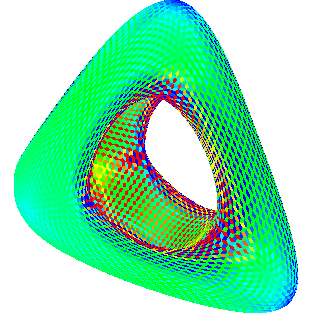
\includegraphics[scale=0.7]{images/genus-mce.png}
    \endminipage\hfill
    \centering
    \minipage[b]{.5\linewidth}
    \centering
    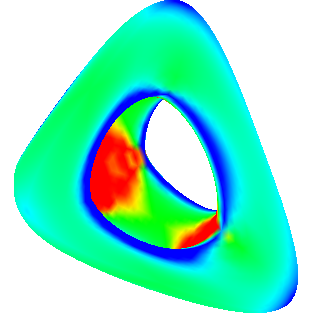
\includegraphics[scale=0.7]{images/genus-mcv.png}
    \endminipage\hfill
    \minipage[b]{.5\linewidth}
    \centering
    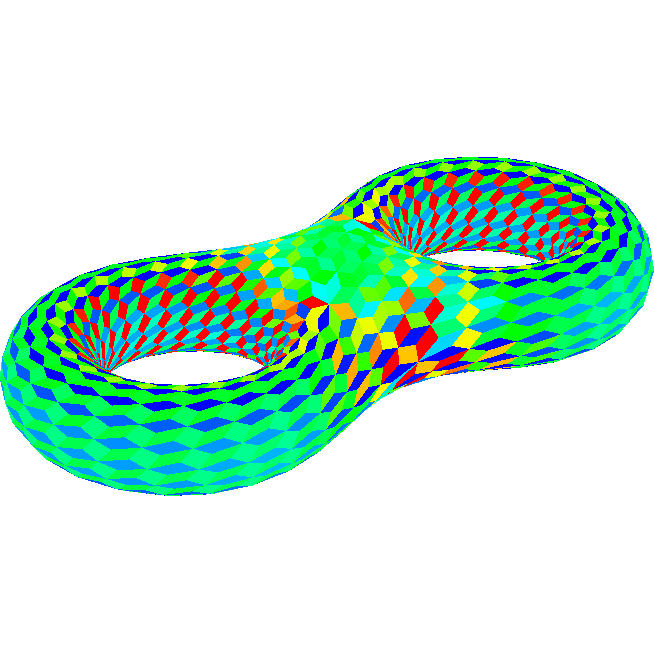
\includegraphics[scale=0.45]{images/eight-mce.png}
    \endminipage\hfill
    \centering
    \minipage[b]{.5\linewidth}
    \centering
    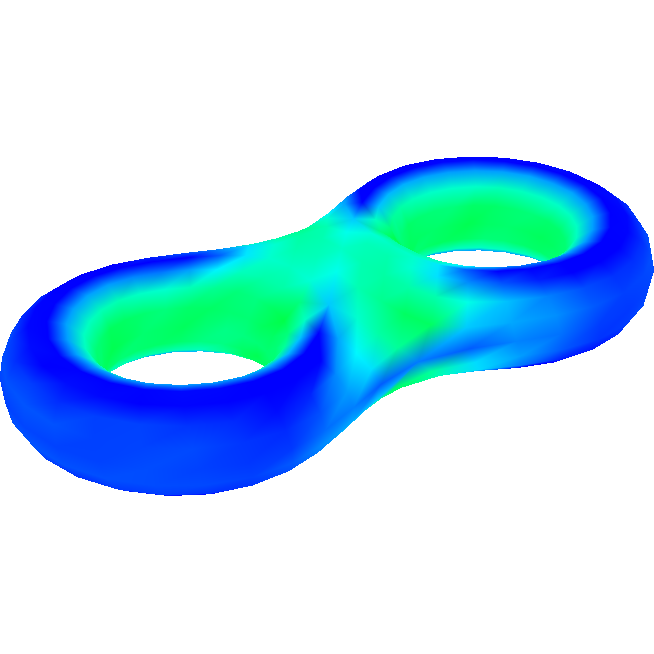
\includegraphics[scale=0.45]{images/eight-mcv.png}
    \endminipage\hfill
    \centering
    \minipage[b]{.5\linewidth}
    \centering
    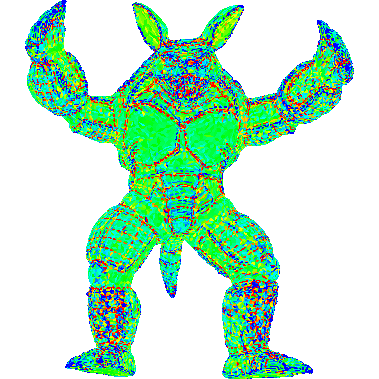
\includegraphics[scale=0.7]{images/armadillo-mce.png}
    \endminipage\hfill
    \centering
    \minipage[b]{.5\linewidth}
    \centering
    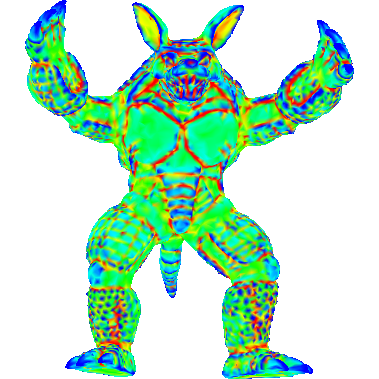
\includegraphics[scale=0.7]{images/armadillo-mcv.png}
    \endminipage\hfill
    \minipage[b]{.5\linewidth}
    \centering
    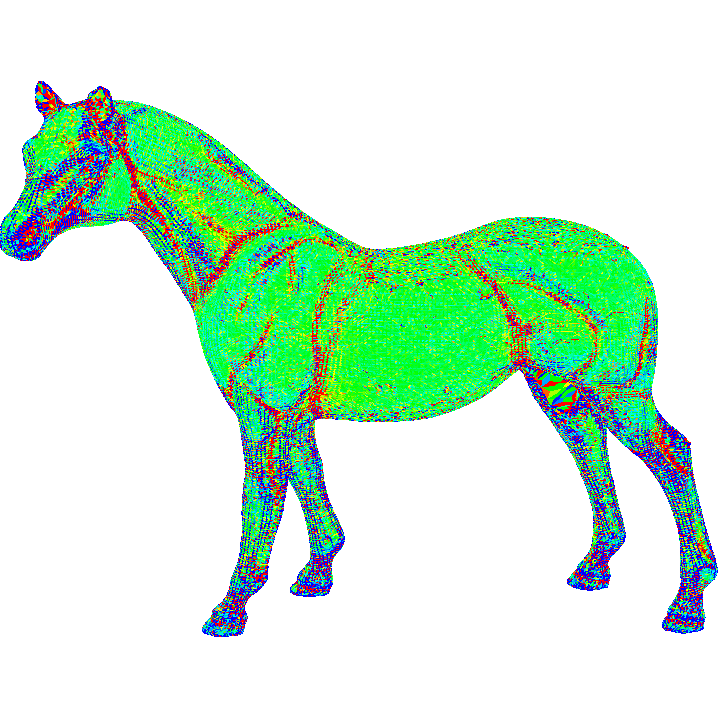
\includegraphics[scale=0.42]{images/horse-mce.png}
    \endminipage\hfill
    \centering
    \minipage[b]{.5\linewidth}
    \centering
    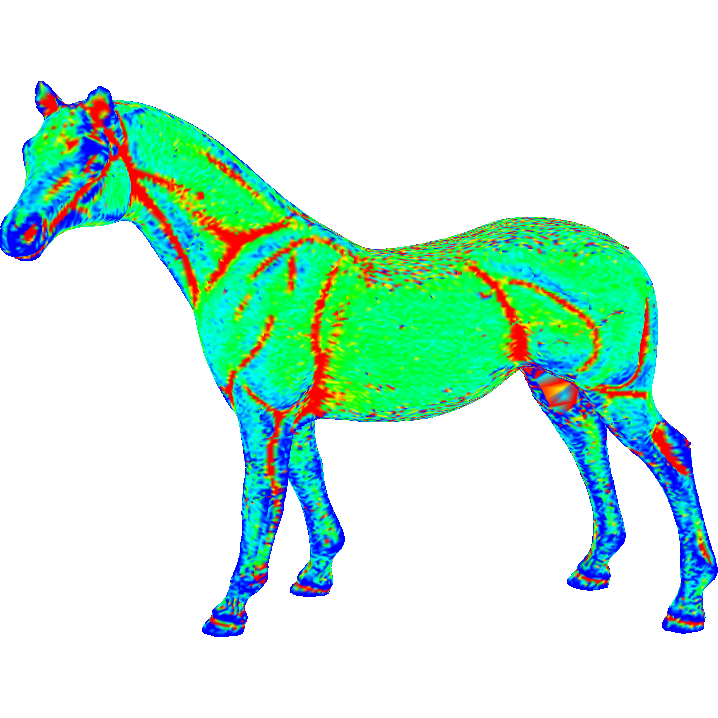
\includegraphics[scale=0.42]{images/horse-mcv.png}
    \endminipage\hfill
    \caption{On the left: Constant mean curvature. On the right: Gouraud mean curvature.}
    \label{fig:comparison-mce-mcv}
\end{figure}